% Dokumentenklasse fuer Artikel waehlen
\documentclass[12pt,onecolumn,oneside,titlepage]{article}

% Deutsche Grundeinstellungen und DIN A4
\usepackage{a4}

% Zur Einbindung von Grafiken mit \includegraphics
\usepackage[pdftex]{graphicx,color}
\DeclareGraphicsExtensions{.pdf,.jpg,.png,.eps,.ps}
\usepackage{graphicx}
\graphicspath{ {images/} }

\usepackage{textcomp,upquote,lmodern,listings}
\usepackage{subcaption}
\usepackage{float}

% Bibliographie mit BibTeX
%\usepackage{natbib}

% Mehrsprachige Bibliographie mit babelbib

\usepackage[english]{babel}
%\usepackage[ngerman]{babel}

\usepackage{babelbib}

% Korrekte Umsetzung von Umlauten
\usepackage[utf8]{inputenc}
\usepackage{times}

\usepackage{hyperref}

% Mathematische Symbole
\usepackage[intlimits,centertags]{amsmath}
\usepackage{amsfonts}
\usepackage{amssymb}
\usepackage{amsmath}

\DeclareMathOperator*{\argmax}{arg\,max}
\DeclareMathOperator*{\argmin}{arg\,min}

% Einrueckung der ersten Zeile eines Absatzes
\setlength{\parindent}{0em}

% Abstand zwischen Absaetzen
\setlength{\parskip}{1.5ex plus0.5ex minus0.5ex}

% Seitenstil
\pagestyle{headings}

% Seitennummerierung
\pagenumbering{arabic}
\setcounter{page}{2}

% Silbentrennungsliste
\hyphenation{native-Hello}

% -- Dokumentenbegin --------

\begin{document}

\title{\bfseries {\Large Proposal Masterthesis}\\[2cm]
      Evaluation of possible improvements to increase sample efficiency of the AlphaZero algorithm.}

\author{\textsc{Colin Clausen}\\[1cm]
        28.11.2019\\[3cm]}

\date{Dozent: \textsc{Prof. Dr.-Ing. Sven Tomforde}\\
      Betreut von: \textsc{Simon Reichhuber}}

% -- Titelseite und Inhaltsverzeichnis erzeugen --------

\maketitle
\setcounter{tocdepth}{2}  % max. Tiefe im Inhaltsverzeichnis
\tableofcontents
%\listoffigures  % optionales Abbildungsverzeichnis
\newpage

\section{Basics AlphaZero}

Beschreibe die Entwicklung von AlphaGo zu AlphaGoZero zu AlphaZero zu MuZero. Gehe auf die Funktionsweise von AlphaZero genauer ein.

\section{Previous work}


\cite{anonymous2020threehead} suggest using a third output head which predicts the win probability after playing every move.


\section{Motivation and possible improvemennts}

The AlphaZero algorithm is a way to attain super human playing strength in arbitrary board games, even ones that before were dominated by human players such as Go.
At least for more complex games like Go this is however still only possible by using very substantial amounts of processing power, thousands of machines clustered together,
making it impossible to leverage the algorithm on hard problems for anyone but the largest organizations.

This motivates the search for improvements that allow to achieve results with lower requirements on computational power, preferably without losing the generality of AlphaZero.
Most time during AlphaZero training is spent on generating example games,
thus it follows that to improve learning speed either more learning has to happen per game or games have to be played out faster.

Previous work has established that large efficiency gains are possible and further improvements shall be systematically investigated and compared to previous improvements as well as a baseline.

\subsection{Means of evaluation}

To be able to experiment fast without massive usage of computing resources simpler games are typically used when evaluating AlphaZero.
Connect 4 is suggested to be used as a primary evaluation game, because classical methods can achieve perfect play and thus evaluation of training progress can be done by judging moves made by AlphaZero in absolute terms.
In similar fashion the game of Hex on a 9x9 board can also be used, for example this is done in \cite{anonymous2020threehead}, as there are datasets of near-perfect play available, this however seems to be a slightly inferior approach, as the network might be penalized
in situations that have multiple optimal moves.

If time and computational resources permit another idea for evaluation on a more complex game would be to implement Chess and judge training progress by the average centipawn loss as measured by a strong Chess engine such as Stockfish, as can be done to judge human players \cite{guid2011using}.
Since Chess is not a solved game this is less accurate than Connect 4, but has the advantage of giving results on a much more challenging domain.


\subsection{Understanding the learning process}

An interesting property of the AlphaZero algorithm is the perceived stability of the training. Other learning systems often struggle to learn two players games in a pure self-play regime, because they get trapped in an endless cycle of learning and unlearning the same mistakes.

A typical way to prevent this normally would be to include earlier iterations of a learner in the learning process, to prevent forgetting previous knowledge.
This was originally done in AlphaGo and AlphaGoZero, however with further work it became clear that even in the AlphaZero regime, with no measures taken at all to prevent forgetting learning works. 
This raises the question of how stable the training truly is. It might be that some amount of forgetting still occurs, just not enough to stop progress.

To research this a dataset of specific game situations could be used, checking which positions are played correctly after every learning iteration. This way it can be compared how every learning iterations adds or removes more understanding of the game to the used neural network.
A better understanding of the learning progress could be valuable to suggest additional ways to speed up training.


\subsection{Suggested improvements to be researched}

playing games as trees - motivated by the huge importance of the accuracy of the game result target
network based features as auxilary targets 
network based features based on a evolutionary algorithm
Squeeze-excite yields improvements (see leela chess zero and the jane street paper), maybe more ideas to increase network efficiency can be taken from papers like mobilenetv3? Less network computations for the same accuracy should translate into quicker training.

\section{Introduction}
\label{sec:intro}

Example introduction section thingy.


\subsection{Related work}

Example subsection about related work, read all of them: \cite{goodfellow2014generative}, \cite{arjovsky2017wasserstein}

\subsubsection{Example formula, also this subsubsection has a label} \label{gansection}

$$ \min_G \max_D V(G, D) = \mathbb{E}_{x \sim p_{data(x)}} [ log D(x) ] + \mathbb{E}_{z \sim p_{noise}(z)}[log(1-D(G(z)))].$$

\subsection{Subsection with a ref to a label}

Here is the ref \ref{gansection}



\section{Images!} \label{sec:exp}

\begin{figure}[H]
 \centering
  \begin{subfigure}{0.3\textwidth}
  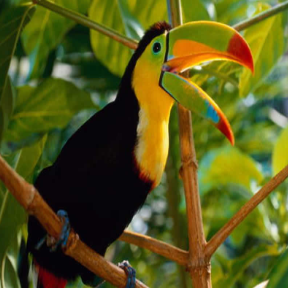
\includegraphics[width=1\textwidth]{bird_HR} 
  \caption{original}
  \end{subfigure}
  \begin{subfigure}{0.3\textwidth}
  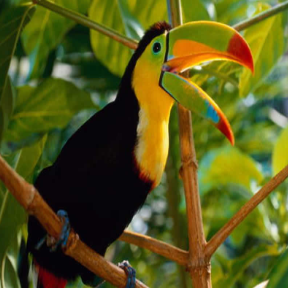
\includegraphics[width=1\textwidth]{bird_HR}
  \caption{SRResNet-MSE}
  \end{subfigure}
  \begin{subfigure}{0.3\textwidth}
  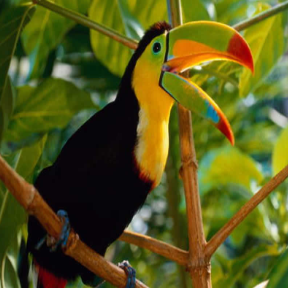
\includegraphics[width=1\textwidth]{bird_HR} 
  \caption{SRResNet-VGG22}
  \end{subfigure}
  
  \begin{subfigure}{0.3\textwidth}
  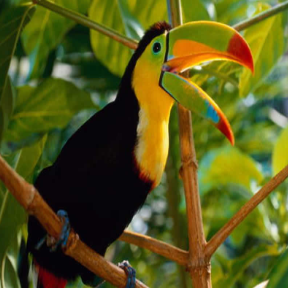
\includegraphics[width=1\textwidth]{bird_HR} 
  \caption{SRGAN-MSE}
  \end{subfigure}
  \begin{subfigure}{0.3\textwidth}
  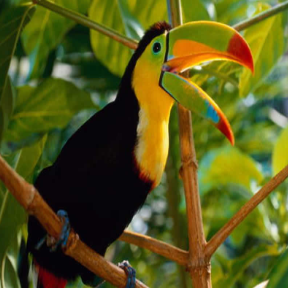
\includegraphics[width=1\textwidth]{bird_HR}
  \caption{SRGAN-VGG22}
  \end{subfigure}
  \begin{subfigure}{0.3\textwidth}
  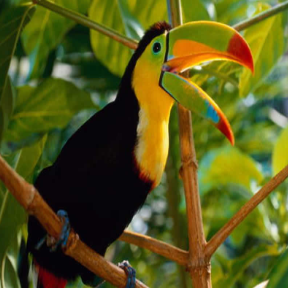
\includegraphics[width=1\textwidth]{bird_HR} 
  \caption{SRGAN-VGG54}
  \end{subfigure}
  \caption{Results on one image from the BSD100 set, best viewn with zoom}
  \label{fig:ex1}
\end{figure}

\subsection{Itemization}

Itemization is a thing.

\begin{itemize}
 \item SRGAN-MSE: $l^{SR}_{MSE}$ uses the standard mean squared error.
 \item SRGAN-VGG22: $l^{SR}_{VGG/2.2}$ uses lower-level features of VGG for the VGG loss
 \item SRGAN-VGG54: $l^{SR}_{VGG/5.4}$ uses higher-level features of VGG for the VGG loss. This is the network that is named simply SRGAN, using higher level features offers the best chance for the network to focus on realistic content of the images, not
 just by local pixel relationships, but in a more global context.
\end{itemize}

\subsection{Tables}

\begin{table}[H]
 \centering
 
 \resizebox{\columnwidth}{!}{
 
 \begin{tabular}{l l l l l l l l l l}
  Set5 & nearest & bicubic & SRCNN & SelfExSR & DRCN & ESPCN & SRResNet & SRGAN & HR\\
  \hline
  PSNR & $26.26$ & $28.43$ & $30.07$ & $30.33$ & $31.52$ & $30.76$ & \boldmath{$32.05$} & $29.40$ & $\infty$ \\
  SSIM & $0.7552$ & $0.8211$ & $0.8627$ & $0.872$ & $0.8938$ & $0.8784$ & \boldmath{$0.9019$} & $0.8472$ & $1$ \\
  MOS & $1.28$ & $ 1.97$ & $2.57$ & $2.65$ & $3.26$ & $2.89$ & $3.37$ & \boldmath{$3.58$} & $4.32$ \\
   \\
  Set14 \\
  \hline
  PSNR & $24.64$ & $25.99$ & $27.18$ & $27.45$ & $28.02$ & $27.66$ & \boldmath{$28.49$} & $26.02$ & $\infty$ \\
  SSIM & $0.7100$ & $0.7486$ & $0.7861$ & $0.7972$ & $0.8074$ & $0.8004$ & \boldmath{$0.8184$} & $0.7397$ & $1$ \\
  MOS & $1.20$ & $1.80$ & $2.26$ & $2.34$ & $2.84$ & $2.52$ & $2.98$ & \boldmath{$3.72$} & $4.32$ \\
   \\
  BSD100 \\
  \hline
  PSNR & $25.02$ & $25.94$ & $26.68$ & $26.83$ & $27.21$ & $27.02$ & \boldmath{$27.58$} & $25.16$ & $\infty$ \\
  SSIM & $0.6606$ & $0.6935$ & $0.7291$ & $0.7387$ & $0.7493$ & $0.7442$ & \boldmath{$0.7620$} & $0.6688$ & $1$ \\
  MOS & $1.11$ & $1.47$ & $1.87$ & $1.89$ & $2.12$ & $2.01$ & $2.29$ & \boldmath{$3.56$} & $4.46$ \\
  
 \end{tabular}
 }
 
 \caption{Comparison of the proposed methods compared to previous methods. SRResNet represents the improvements gained from simply using a deeper network, while SRGAN represents combining the deeper network with the proposed perceptual loss.}
 \label{tab:results}
 
\end{table}


\section{Text with footnote}
Since the paper was published an independent implementation of SRGAN has been created \footnote{https://github.com/aitorzip/PyTorch-SRGAN}.


% -- Literaturverzeichnis --------

\bibliographystyle{plain}     % nummeriere Zitate [1], [2], ...

% Quellenangaben stehen in einer separaten BibTeX-Datei Seminararbeit.bib
\bibliography{document}

\end{document}
